\documentclass[12pt]{article}
\usepackage{amsmath}
\usepackage{graphicx}
\usepackage{enumerate}
\usepackage[authoryear,numbers]{natbib}
\usepackage{graphicx}
\usepackage[english]{babel}
\usepackage[colorlinks=true, allcolors=blue]{hyperref}
\usepackage{caption}
\usepackage{subcaption}
\usepackage{placeins}
\usepackage{hyperref}
\usepackage{float}
\usepackage[utf8]{inputenc}
\usepackage{hyphenat}
\tolerance=1000
\usepackage{url}
\usepackage{textcomp}
\usepackage{tikz}
\usepackage{hyphenat}
\usepackage{Sweave}
\bibliographystyle{apalike}
\newcommand{\blind}{1}

% DON'T change margins - should be 1 inch all around.
\addtolength{\oddsidemargin}{-.5in}%
\addtolength{\evensidemargin}{-1in}%
\addtolength{\textwidth}{1in}%
\addtolength{\textheight}{1.7in}%
\addtolength{\topmargin}{-1in}%

\begin{document}
\Sconcordance{concordance:ms.tex:ms.Rnw:1 58 1 1 816 56 1 1 26 1 2 2 1 1 29 1 2 221 1 %
1 8 121 1 1 18 24 1}

\def\spacingset#1{\renewcommand{\baselinestretch}%
{#1}\small\normalsize} \spacingset{1}


\if1\blind
{
  \title{\bf Mechanistic models for panel data: analysis of ecological experiments with four interacting species}
\author{Bo Yang\\Department of Biostatistics, University of Michigan \\
        Jesse Wheeler\\Department of Statistics, University of Michigan \\
        Aaron A. King\\Department of Ecology and Evolutionary Biology \& \\ Center for the Study of Complex Systems, University of Michigan\\
        Edward L. Ionides\\Department of Statistics, University of Michigan}
  \maketitle
} \fi


\if0\blind
{
  \bigskip
  \bigskip
  \bigskip
  \begin{center}
    {\LARGE\bf Mechanistic models for panel data: analysis of ecological experiments with four interacting species}
\end{center}
  \medskip
} \fi




\bigskip
\begin{abstract}
In ecological research, panel data, often comprising multi-magnitude time series, presents unique analytical challenges due to its high dimensionality. This study employs the PanelPOMP framework and the Panel Iterated Filtering (PIF) method to explore the practicality and advancement of mechanistic model development for such complex datasets. Mechanistic models, especially valuable in ecological research, allow for quantitative analysis and deeper understanding of dynamic systems. However, they are often constrained by the non-Gaussian nature of ecological data. Our study applies these methods to the Daphnia panel data, consisting of independent time series with 10 data points each, to derive parameters that minimize the Akaike Information Criterion (AIC). The comparison of AIC values across models reveals the significant impact of alga, the prey of Daphnia, and parasite on their population dynamics which is observed in the SIRPF model highlights this relationship. The panelPOMP framework's ability to handle complex panel data analysis is demonstrated, emphasizing its utility in uncovering latent processes not captured by traditional models. However, the study also discusses limitations and interpretations of mechanistic models and PanelPOMP framework in ecological data analysis.
\end{abstract}

\noindent%
{\it Keywords:}  Panel Iterated Filtering; SIRPF model; PanelPOMP; Daphnia. 
\vfill

\newpage
\spacingset{1.9} % DON'T change the spacing!
\section{Introduction}
\label{sec:intro}

Ecological experiments contain many elements or processes that are difficult to observe, models that can describe both observable and unobservable processes to explain the whole ecological experiment are necessary. As a mathematical description of the elements forming a system, mechanistic modeling can describe the mutual interactions between elements in the system and their interactions with the environment \citep{Stalidzans2020}. Utilizing the established process, they elucidate the actions of hidden mechanisms \citep{Duarte2003}. The purpose of mechanistic modeling in ecology involves employing mathematical models to depict the development and interaction of dynamic systems. This quantitative tool allows researchers to evaluate the explanatory potential of various conceptual models and measure the magnitude of pertinent parameters. Mechanistic modeling has been widely employed in social sciences, industrial engineering, and physics for an extended period. Improved computational capabilities now make it more effective. Traditional time series analysis offers limited explanatory power due to the nonstationary, nonlinear, and stochastic nature of ecological information. Despite the creation of theoretical models for the data, connecting theories with data continues to be a challenging task. As a result, ecological mechanical modeling cannot solve most of the problems on a wide scale, but rather, only a limited range of the problems \citep{levin1992problem}.\\

Panel data, sometimes referred to as longitudinal data, is composed of multiple time series. Each of these time series, which may be multivariate, contains a series of observations collected from a separate entity  \citep{Carles2020}. In ecology, panel data is a traditional data form that researchers gather to mitigate the impact of random variations throughout experiments, so that it can more accurately measure changes in experimental objectives and control the variables needed to achieve experimental goals. Due to the non-linear characteristics of ecological data, the analysis of panel data entails a high-dimensional structure. Such features diminish the explanatory power of traditional time series analysis and certain Monte Carlo inference techniques \citep{johnstone2009statistical}. The goal of this study is to investigate the practicality of employing mechanistic models on ecological panel data using the panelPOMP structure.\\

The PanelPOMP approach modifies the partially observable Markov Process model to accommodate panel data by constructing a POMP model for each individual component \citep{King2016}. This method enables the determination of whether the parameters within the selected mathematical model are shared or distinct throughout the panel, by computing the highest log likelihood for all potential combinations through the use of panel iterated filtering. Stemming from iterated filtering \citep{King2016} applied to a singular nonlinear stochastic time series, panel iterated filtering not only filters within each series but also cycles across the panel to achieve the best likelihood. This enables the application of mechanistic models to panel data while preserving its intricate dimensionality.\\

In this research, we will show the advancement of the panelPOMP model by analyzing the Daphnia panel data generated in the experiment of Searle et al. \citep{Searle2016}. The research group of Searle et al. collected panel data on the population densities of different species of Daphnia under different conditions, and interpret how invasive Daphnia species (\textit{lumholtzi}) affect the response of native Daphnia species (\textit{dentifera}) to parasites with panel data \citep{Searle2016}. In their lab experiment, they generated standard ecological panel data featuring various independent trials under the same experimental conditions, with each consisting of a brief, nonlinear, and nonstationary time series. Conventional mechanistic theories cannot directly interpret these observations. Utilizing the panelPOMP approach allows for the combination of theoretical models and empirical data, enabling the extraction of the comprehensive information found in each individual time series \citep{Carles2020}.\\

For a more in-depth examination of the concealed processes in the panel data, this research incorporates the Susceptible-Infected-Recovered-Food-Parasite (SIRPF) model - within the panelPOMP framework. After applying the model to the Daphnia panel data, the maximum log-likelihood and best parameter estimates are determined via an iterative filtering approach. These findings are subsequently compared to discover a more accurate and appropriate model for the given data. The superior performance of the SIRPF model implies that the population density of alga \textit{Ankistrodesmus falcatus}, which is Daphnia's prey, impact the dynamics of both species of Daphnia. It is worth noting that the population density of alga is neither observable nor recorded in the experiment. That implies the mechanistic models under panelPOMP potentially better explain the latent process and show the importance of unobservable processes \citep{Edwards2012}. At the same time, the panelPOMP framework provides an estimation of the parameters in the model, which helps to understand the hidden mechanisms in the ecological system \citep{Carles2020}. Based on the estimation, a detailed interpretation of relationship between invasive host and native host with presence of parasite is explaned.\\

Our objective is to evaluate the explanatory capabilities of two traditional ecological models when applied to the Daphnia panel data, and to estimate the parameter sets for a more accurate depiction of the hidden mechanisms within the ecological system. By analyzing Daphnia panel data, we hope to show the limitations and interpretations of mechanistic models in dealing with ecological data. Additionally, the later section will further discuss how the panelPOMP framework and PIF contribute to overcoming the inherent challenges associated with fitting ecological models.


\section{Study System}
\label{sec:studysystem}

The dynamics of our study are derived from the Searle's comparison experiment, which focuses on two Daphnia species: Daphnia \textit{dentifera Forbes}, natively prevalent in North American stratified lakes \citep{searle2016salinization}, and Daphnia \textit{lumholtzi Sars}, an invasive species originating from Africa, Asia, and Australia. D. lumholtzi, first observed in North America in the 1990s, has rapidly expanded across the United States, impacting native species and ecosystem dynamics \citep{havel1993daphnia}. These Daphnia species, referred to as the native and invasive hosts, are bred in controlled laboratory environments using isofemale lines. For their experiments, six clones of each species were selected to eliminate selection bias \citep{Searle2016}.\\ 

The dynamics also involves \textit{Metschnikowia bicuspidata}, a parasitic fungus predominantly infecting the native host. This parasite, ingested as spores by Daphnia, aggressively affects the host's fecundity and longevity \citep{duffy2010temporal}. The parasite's presence is identifiable by the opaqueness it causes in normally transparent hosts, with spore release upon host death. Searle's study utilized a M. bicuspidata strain from Baker Lake, Michigan, with consistent infectivity and virulence characteristics in different samples \citep{Searle2016}. The final species in our study is \textit{Ankistrodesmus falcatus}, a green alga that serves as the primary food source for Daphnia. \textit{Ankistrodesmus falcatus} is a globally distributed freshwater chlorophyte, is known for its role in aquatic communities and has been utilized in ecological research due to its nutritional properties \citep{arnold1971ingestion}. Its significance is particularly evident in controlled experimental settings where the growth conditions and feeding rates of Daphnia species can be closely monitored and manipulated \citep{martinez1994effect}.\\

Drawing upon the empirical findings from Searle's laboratory, it was observed that while the two Daphnia host species exhibited comparable resource acquisition rates, the invasive species demonstrated a more rapid reproductive cycle \citep{Searle2016}. This observation suggests a potential competitive advantage for the invasive species. Building on these insights, Searle and colleagues structured the ecological system we analyze here, focusing on dynamics at the community level. Their approach involved a mesocosm experiment that varied species composition and parasite presence. The experimental design was a 3x2x1 factorial arrangement, incorporating three species combinations (native only, invasive only, or both existing species), two parasite exposure scenarios (exposed or unexposed), and a single algal food source. This design enabled an in-depth analysis of the invasive host's impact on native populations, manifesting either directly through competition for resources, indirectly via the amplification of a mutual parasite, or through a reduction in parasite effects.\\

In essence, the impact of an invasive Daphnia \textit{lumholtzi}, particularly in terms of resource competition like food, can be significant. This scenario would lead to a decreased survival rate of the native host in the presence of the invasive species, irrespective of parasite interference. This effect is quantifiable through the ratio of natality to mortality in the native host population. Conversely, should the invasive species primarily influence the native host indirectly via interactions with parasites, a different pattern emerges. Here, the survivability of the native host is expected to be lower in scenarios involving both the parasite and the invasive host, as opposed to situations where the native host is only affected by the parasite. This effect is quantifiable through the ratio of natality to mortality in the native host population as well.\\

\subsection{Non-parasitized Dynamics}
This research stratifies the ecological dynamics above into two analytical categories delineated by parasitic presence. Under the 'Non-parasitized Dynamics' classification, three experimental groups of Daphnia species—solely native, solely invasive, or a combined population—are statistically analyzed. This categorization facilitates a quantitative assessment of the interaction dynamics between native and invasive Daphnia species, particularly in environments not influenced by parasitic interactions.\\

In the Non-parasitized level, indoor mesocosms were used \citep{Searle2016}, each comprising a 18.9 L bucket with 15 L of high-hardness COMBO media. The experimental design involved 10 replicates for single-species treatments, and 9 replicates for mixed-species treatment. A nitrogen-to-phosphorus ratio of 25:1 was established, and each mesocosm was seeded with 2.5 $\times$ $10^8$ cells of \textit{Ankistrodesmus falcatus}. The laboratory conditions included an average temperature of 23.27$^\circ C$ ($\pm$0.2) and a 16-hour light, 8-hour dark cycle. For single-species treatments, either 45 native or invasive Daphnia hosts were added, representing six genotypes per species to eliminate the selection bias. In mixed-species treatments, 35 native and 10 invasive hosts were introduced, simulating early invasion stages.\\

\subsection{Parasitized Dynamics}
Parasitized dynamics is employed with a key difference, which is the presence of the parasite \textit{Metschnikowia bicuspidata} . Based on the same setup of Non-parasitized Dynamics, after a 4-day acclimation period in the mesocosms, hosts are exposed to parasites, with spore counts set at 25 per mL in parasite-exposed treatments. This category allows for the investigation of the impact of parasites on the interaction dynamics between native and invasive Daphnia species, particularly how parasitism influences competition and survival rates. This approach complements the "Non-parasitized Dynamics" by providing a contrasting scenario where parasitic factors are at play, thereby enriching the understanding of ecological interactions under the presence of parasite.\\

\subsection{Data Collection and Visualization}
Population densities and infection prevalence(if exists) were quantified every five days, beginning a week after the experiment started. On each sampling day, mesocosms were thoroughly mixed, and a 1-liter sample was removed and replaced with fresh COMBO media. The samples were concentrated using a 153-$\mu m$ mesh and the Daphnia were counted under a microscope. For each Daphnia, species (native or invasive), infection status, age, and sex were determined. Regular stirring of mesocosms ensured resuspension of algae and parasites. Algal and nutrient levels were supplemented bi-weekly, with COMBO media added as necessary. The experiment concluded after 52 days, totaling 10 sampling sessions \citep{Searle2016}.\\

As juveniles rarely exhibit clear signs of infection, only adult Daphnia were used for quantifying effects in both Non-parasitized and Parasitized Dynamics to minimize information bias. Figures below illustrates these dynamics, with the figure 1 depicting Non-parasitized Dynamics (mixed-species) where changes in native and invasive host densities reflect direct resource competition, for example, food alga \textit{Ankistrodesmus falcatus}. Figure 2 shows Parasitized Dynamics, where the interplay of susceptible and infected Daphnia of different species is further influenced by parasites, complicating the variation of susceptible and infected Daphnia of different races, which makes it difficult to directly analyze the sources of influence on their variation. Non-parasitized Dynamics will be analyzed at the first place to help understand the effect of resource competition in mixed-species. And based on this result, the correlation between native host and invasive host in Parasitized Dynamics will be further explored.

\begin{figure}[htbp]
\centering
\begin{subfigure}[b]{\linewidth}
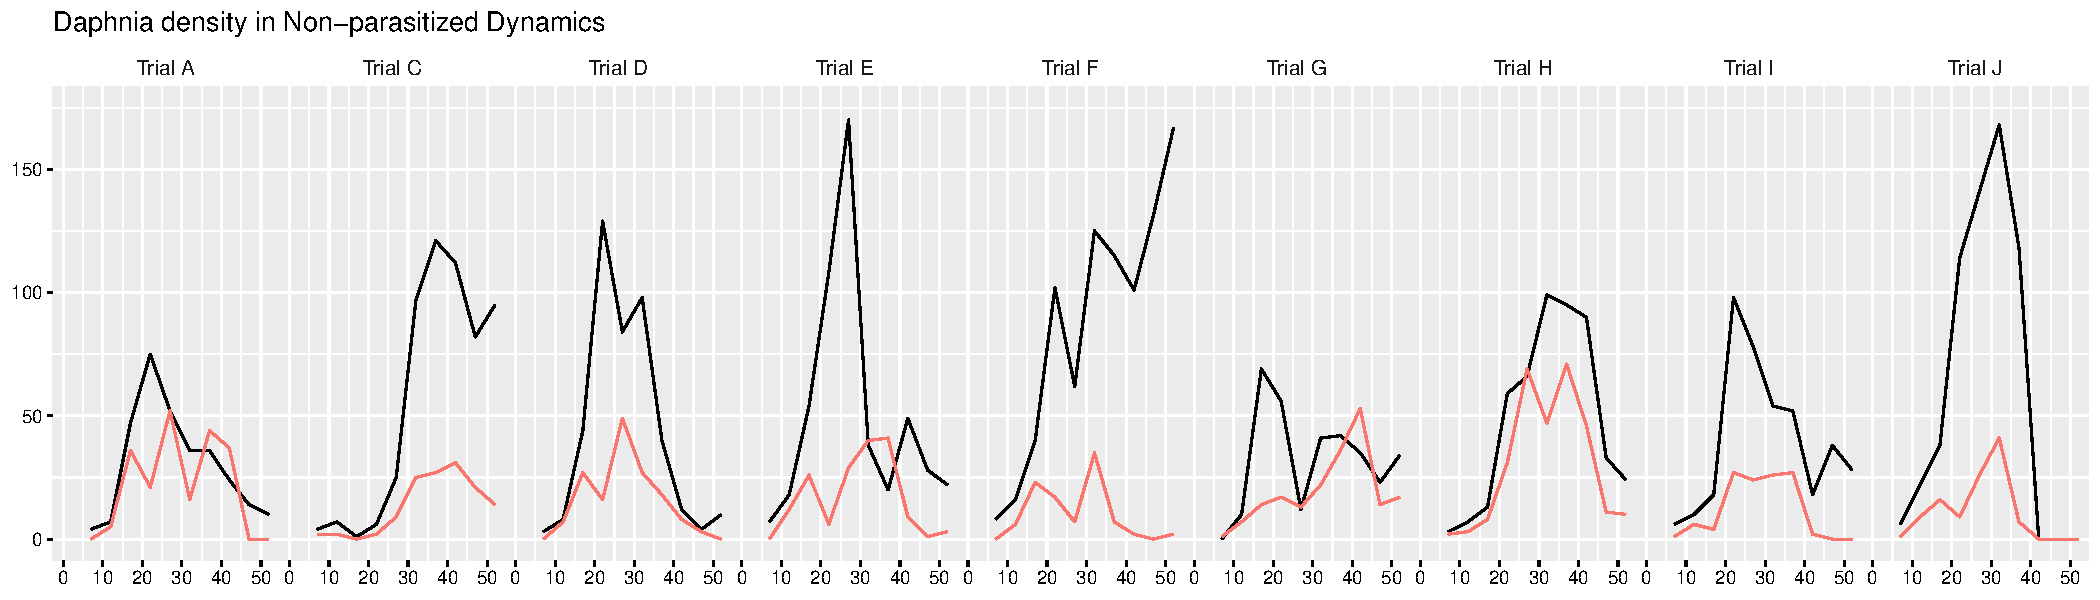
\includegraphics{ms-002}
\caption{Plot of density of hosts in dynamics including both native and invasive host species of Daphnia. The trail A to J represents different buckets in the experiment}
\end{subfigure}
\begin{subfigure}[b]{\linewidth}
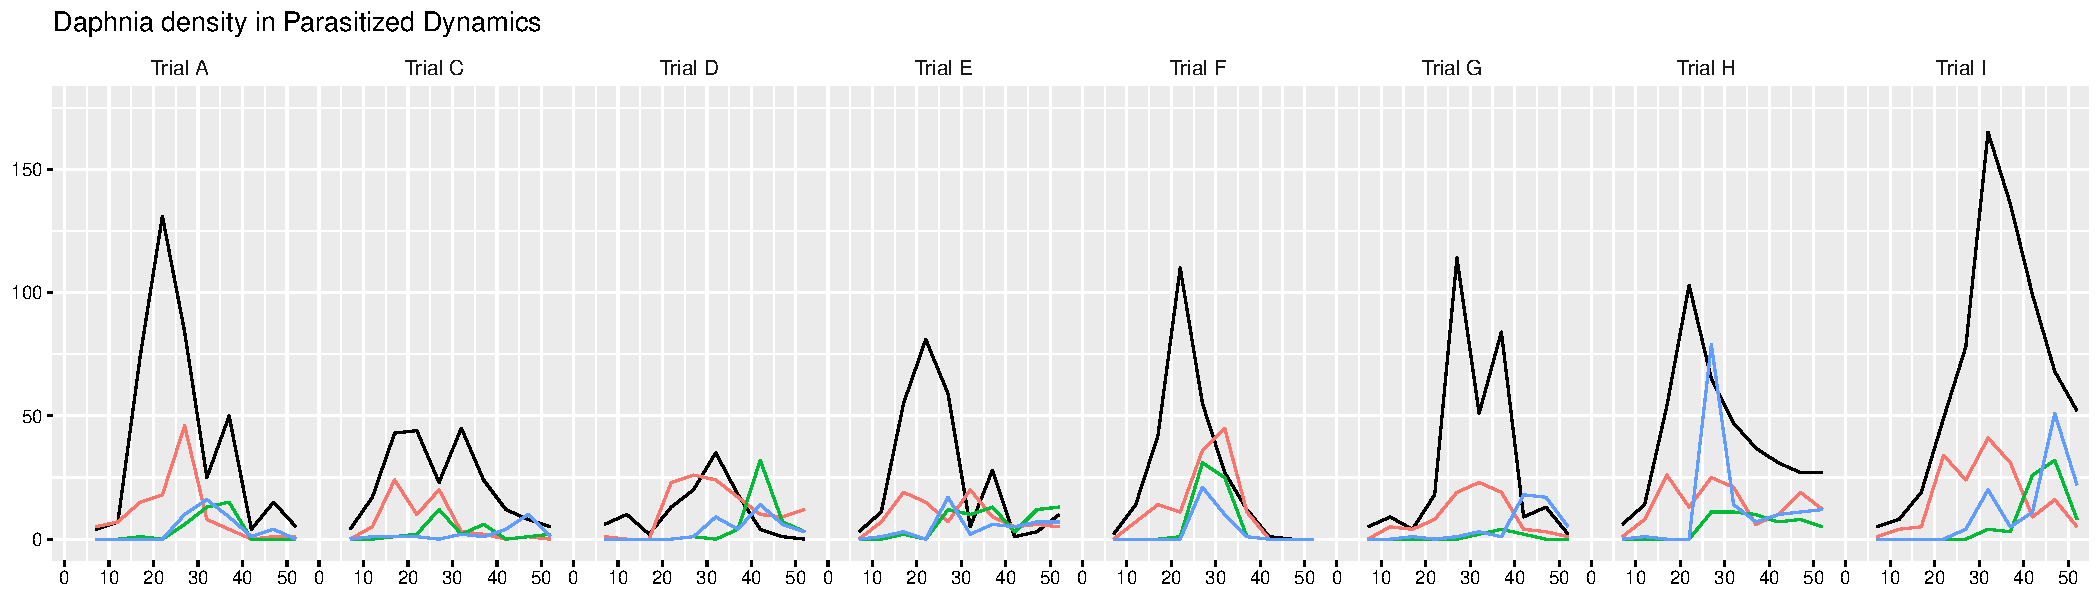
\includegraphics{ms-003}
\caption{Plot of density of hosts in dynamics including both native and invasive host species of Daphnia. The trail A to J represents different buckets in the experiment}
\end{subfigure}%
\end{figure}

\section{Methodology}
\label{sec:meth}
\subsection{Partially Observed Markov Processes}
Frequently, we lack a comprehensive understanding of the underlying mechanisms that drive the evolution of a natural system. For example, the precise number of individuals who are exposed to a disease or the density of alga at any given time is typically unknown. To address these issues of missing information, we can utilize partially observed Markov (POMP) models. These models combine both latent and observable processes which are reliant on each other \citep{bhadra2011malaria}.\\

The application of POMP models spans various fields, including epidemiology, ecology  \citep{king2022markov}, and finance \citep{welton2005estimation} where they are used to infer the dynamics of complex systems from partial observations. For instance, in epidemiological studies, POMP models are instrumental in estimating disease transmission rates and predicting future outbreaks by modeling the spread of infectious diseases when only a fraction of cases are observed \citep{xue2020data}. Similarly, in ecology, these models help in understanding animal population dynamics and migration patterns based on limited or sporadic sighting data \citep{wood2001partially}.\\

Methodologically, POMP models are analyzed using a suite of computational techniques. Sequential Monte Carlo methods, such as particle filters, are commonly employed for state estimation and parameter inference in these models \citep{bhadra2011malaria}. These methods involve simulating a large number of potential realizations of the latent process and updating these simulations as new observations become available, thereby approximating the posterior distribution of the state given the data \citep{King2016}. Additionally, techniques like iterated filtering and particle Markov chain Monte Carlo are used for parameter estimation and model calibration.\\

With the random variables $Y_{0:N}$ which are the observable states process, the measurement model is $f_{Y_n|X_n}(y_n|x_n)$, and the collected data $y_{0:N}$ are observations of this process. We suppose random variables $X_{0:N}$ represent the latent states, where $X_0$ represents the initial state of the latent process, $f_{X|X_{n-1}}(x_n|x_{n-1})$. We assume that each $Y_n$ depends only upon the latent process at time $n$, $X_n$, and is conditionally independent of the other variables representing the measurement and latent processes, $Y_{n-1}$ and $X_{n-1}$, where $1 \leq n$. Together, $X_{0:N}$ and $Y_{0:N}$ form our POMP model. POMP models are vital in situations where we encounter incomplete or noisy measurements of a latent, unobserved Markov process. These models, also known as hidden Markov models or state space models, are particularly adept at handling time series data where observations are only partial or indirect representations of the underlying state of the system. Their strength lies in the combination of a latent process, which evolves according to Markov dynamics, and an observation process, which relates the latent states to the actual data observed.\\


\subsection{PanelPomp Framework}
In a panel data set containing K independent time series, K entities are represented by the symbols $1,2,...,K$, with N periodic observations collected for each unit $(t_1,t_2,...,t_{N})$. A stochastic observable process, denoted as $y_{k,1},...,y_{k,N}$, generates these measurements. PanelPOMP is an adaptation of the partially observable Markov process (POMP) tailored for panel data analysis. It entails developing a POMP model for each entity and employing the Panel Iterated Filtering (PIF) method to achieve the highest log-likelihood. Based on the POMP framework, a process and a measurement model were devised for every time series unit. The measurement model elucidates how the potential real population density generates observable time series data with the measurement density $f_{Xn|Xn-1}(x_n|x_{n-1};\theta)$, while the process model portrays the actual population's dynamics through the one-step transition density $f_{Xn|Xn-1}(x_n|x_{n-1};\theta)$. Ultimately, the joint density equals the initial density multiplied by the product of the process and measurement models for each state.\\

The PanelPOMP framework demonstrates a strong capability in handling ecological panel data due to its ability to model complex, time-varying processes within and across multiple ecological units \citep{Carles2020}. It efficiently integrates mechanistic models that capture underlying ecological dynamics with statistical inference methods, accommodating variability and correlations across units. This framework is adept at dealing with incomplete or noisy observational data, typical in ecological studies, providing robust estimates and predictions that are crucial for understanding and managing ecological systems.\\


\subsection{Likelihood of models and PIF}

In statistical inference challenges, likelihood frequently serves as the basis for estimating parameters and selecting models. Considering a model parameterized by vector $\theta$ within the $m$-dimensional parameter space $\Theta_m$, the likelihood function represents the combined probability density of the dataset, $y_{1:N}$, at $\theta$:
        \begin{equation}
        \mathcal{L}(\theta) = f_{Y_{1:N}}(y_{1:N}; \theta)
        \end{equation}
The goal is to get the estimation of $\theta$, $\hat{\theta}$ that maximizes the likelihood function $\mathcal{L}(\hat{\theta})$, or log-likelihood function $\mathbf{\ell}(\hat{\theta})$.

An ecological model's effectiveness in tracking disease spread hinges on its capability to predict cases or incidence rates. This capability is inherently tied to our trust in the model's precision in forecasting and our grasp of the temporal changes in latent states. As a result, we encounter two interrelated issues: ascertaining the distribution of $X_{n}$ at time $n$ based on $y_{1:n}$, and pinpointing parameter values, $\hat{\theta}$, that maximize the data likelihood. These processes are commonly respectively concluded as the filtering process and the inference process.\\

Working with POMP models can prove difficult due to the complexity of formulating both the likelihood function and transition density in intricate settings. To address this issue, several techniques have been devised, including the particle filter. Utilizing the particle filter method, it is only necessary to supply data, initial density simulators, single time-step transition density simulators for the latent process, and an evaluator for the observation process density reliant on the hidden process in order to achieve maximum likelihood estimates.\\

To implement the particle filter, we start by initializing $M$ particles at time 1, where $\{ X_1^m; m \in 1:M \}$. All with the required latent state detail and a vector of parameter values, $\theta$. As a result, for every time step n, where $n \in $ [$N$], we advance the each particle by doing the one-step random walk based on transition density, resulting in a set of particles that represents the prediction distribution at time n, which can be represented as $f_{X_n|X_{n-1}}(\cdot | X_{n-1}^m; \theta)$. Next, we assign weights to the particles based on the measurement density to obtain an ensemble that represents the filtering distribution at time n, where the new weight is calculated via $w_{n,m} = f_{Y_n|X_n}(y_n | x_n^m)$. Finally, we reassign the particles based on their weights to generate a new set of particles that represents the filtering distribution, which can then be used to estimate model parameters swarm based on the maximum likelihood \citep{5}. The particle filter is particularly useful in situations where both the likelihood function and transition density are difficult to calculate analytically.\\

As we know, the measurement process variables are mutually independent. In the mean time, the latent process states are dependent to one other. We also notice that the weight we assign to the particles will vary among different particles, which makes the calculation hard. As M to be large enough, we may approximate the weight of each particle to be the mean value of the to calculate the log-likelihood. Based on such fact, we can summarize as following:
         \begin{flalign}
          \mathcal{L}(\theta) &= f_{Y_{1:n}}(y_{1:N}; \theta) \\
         & = \prod_{n=1}^N f_{Y_{n} | Y_{1:n-1}}(y_n | y_{n-1}; \theta) \\
         & = \prod_{n=1}^N f_{Y_n | X_n}(y_n | x_n ; \theta)\\
         & \approx \prod_{n=1}^N \frac{1}{M} \sum_{m = 1}^M f_{Y_n|X_n}(y_n | x_n^m) 
         \end{flalign}
The particle filter, a form of Sequential Monte Carlo method, is instrumental in processing partially observed Markov processes within complex statistical models \citep{ionides2006inference}. This technique hinges on the generation of multiple, simulated "particles" that each represent a potential state of the latent process \citep{ionides2011iterated}. As new observational data becomes available, these particles are updated and assigned weights proportional to their likelihood of representing the true latent state, considering the observed data.\\

This weighting system is key to the particle filter's efficacy. It allows for the approximation of the distribution of the latent process at any given point in time, as well as the conditional likelihood of the observed data given the model. Essentially, the particle filter distills a complex, high-dimensional problem into a manageable computation by focusing on the most probable states of the latent process, as indicated by the observed data.\\

Panel Iterated Filtering (PIF) extends the improved iterated filtering algorithm, originally developed for time series data, to panel models \citep{Carles2020}. This method is particularly effective in exploring parameter spaces in complex, nonlinear, non-Gaussian models.  It does this by introducing random perturbations to the model parameters and utilizing a particle filter to explore the parameter space at each iteration. The convergence to a maximum likelihood estimate is achieved through procedures that iterate this search over the parameter space while diminishing the intensity of perturbations.\\

PIF's functionality is especially valuable in analyzing complex dynamical systems where the standard modeling approaches may fall short due to the intricacies of the data and the underlying processes. The ability of PIF to handle high-dimensional parameter spaces and its flexibility in managing different types of data structures make it a robust tool for statistical inference in complex models, particularly those encountered in ecological and epidemiological studies.\\

\section{Mechanistic models}
\label{sec:mecmod}
Mechanistic models are highly effective in understanding ecological dynamics due to their ability to incorporate detailed biological processes and interactions within ecosystems \citep{young1998data}. These models simulate the causal mechanisms underlying ecological phenomena, offering insights into complex ecological processes that are often difficult to observe directly. By integrating empirical data with theoretical principles, mechanistic models enable the prediction and analysis of ecological outcomes under varying conditions. This makes them invaluable tools for addressing challenges in ecology \citep{mouquet2015predictive}.\\


In mechanistic modeling of dynamic systems, the foundational step involves the formulation of differential or difference equations that encapsulate the temporal evolution of the system. This approach is pivotal in time series analysis using mechanistic models, which primarily aims to assess the model's adequacy in capturing the dynamics of the system and, upon validation, estimate unknown parameters that govern these dynamics \citep{breto2009time}. The complexity in such models often arises from intrinsic stochasticity, nonlinearity, and the presence of noisy and incomplete observational data, features that are particularly prevalent in biological sciences \citep{wilkinson2018stochastic}.\\

To analyze the dynamics of Parasitized and Non-parasitized systems, the Susceptible-Infected-Recovered-Food-Parasite (SIRPF) model, an adaptation of the SIR model \citep{weiss2013sir}, is utilized. This model integrates the aspects of food and parasites, unlike the classical SIR model, to more accurately reflect the interactions between native and invasive hosts in the context of resource availability and parasitic influence. The SIRPF model incorporates these factors as quantitative latent state variables, enabling a more comprehensive understanding of the system's dynamics. In the meantime, the ecological processes of Daphnia can be viewed as a Markov process, where the population of Susceptible and Infected individuals is observable, while the amount of food and parasites represent unobservable latent states. Utilizing panel data on Daphnia, the PanelPOMP framework becomes a valuable analytical tool \citep{Carles2020}. Despite the lack of direct measurement data for these latent states, PanelPOMP, which has proven efficiency in analyzing ecological panel data, facilitates a robust analysis of these dynamics, effectively handling the complexities inherent in ecological systems.\\

The SIRPF model describes the dynamics of the Susceptible($S$), Infected($I$), Recovered, Food($F$), and Parasite($P$) populations as the following graph and model show: 

\usetikzlibrary{positioning}
\usetikzlibrary {arrows.meta}
\usetikzlibrary{shapes.geometric}

\begin{figure}
\begin{center}
%%%%% SEAIR diagram
\resizebox{8cm}{!}{
\begin{tikzpicture}[
  square/.style={rectangle, draw=black, minimum width=0.5cm, minimum height=0.5cm, rounded corners=.1cm, fill=blue!8},
  rhombus/.style={diamond, draw=black, minimum width=0.05cm, minimum height=0.05cm, fill=purple!8,aspect = 1,inner sep=0cm},
  travel/.style={circle, draw=black, minimum width=0.5cm, minimum height=0.5cm, fill=green!8},
  report/.style={shape=regular polygon, regular polygon sides=8, draw, fill=red!8,minimum size=0.6cm,inner sep=0cm},
  bendy/.style={bend left=10},
  >/.style={shorten >=0.25mm}, % redefine arrow to stop short of node
  >/.tip={Stealth[length=1.5mm,width=1.5mm]} % redefine arrow style
]
\tikzset{>={}}; % this is needed to implement the arrow redefinition

\node (S) at (-0.5,-0.25) [square] {$S$};
\node (I) at (4.5,-0.25) [square] {$I$};
\node (P) at (2.5,0.75)  [rhombus] {$P$};
\node (R) at (3.5,2)[travel] {$R$};

\node (F) at (4.5,4.5) [report] {$F$};


\draw [->] (F) --  (R);
\draw [->] (P) --  (R);
\draw [->] (S) -- (R);
\draw [->] (I) -- (R);

\draw [->] (F) -- (S);
\draw [->] (F) -- (I);

\draw (S) edge[loop left] (S);
\draw (F) edge[loop above] (F);

\draw [->, bendy] (S) to  (I);
\draw [->, bendy] (I) to  (S);
\draw [->, bendy] (P) to (I);
% \path [->] (S) edge (I) 
%            (P) edge (I);
\draw [->, bendy] (I) to (P);
\end{tikzpicture}
}
\end{center}
\vspace{-5mm}
\caption{A flow diagram for the SIRPF model. Apart from the quantified states above, the graph includes $R$ state, which represents deadth status. For Daphnia either dentifera or lumholtzi, susceptible, infected Daphnia and food retain the ability to produce offspring, which is represented in the graph as a self-recycling of $S$ and $F$, as well as transaction from $I$ to $S$. Some susceptible Daphnia get infected by parasites, transitioning from $S$ to $I$. Both susceptible and infected Daphnia contribute to the $R$ state upon death, releasing surviving parasites back into the environment. And the parasites continue to impact other individuals and get into another cycle. Food is consumed by both $S$ and $I$ individuals. Over time, elements in $F$ and $P$ also transit to the $R$ state.}
\label{fig:flow_SIRPF}
\end{figure}

{
\small
\begin{align}
&d S(t) = r F(t)\left(S(t)+\xi I(t)\right)dt - \theta_{S}S(t) dt - p f_{S} S(t) Pdt - \delta S(t)dt + S(t) d\zeta_{S},\\
&d I(t) = p f_{S} S(t) Pdt - \theta_{I} I(t)dt - \delta I(t)dt + I(t) d\zeta_{I},\\
&dF(t) = \alpha F(t)\left(1-\frac{F(t)}{K_F}\right)dt - \gamma F(t) \left(S(t)+\xi I(t)\right) dt - \delta F(t) dt + \mu dt + F(t) d\zeta_F,\\
&d P(t) = \beta d I(t)dt - f_{S} S(t) P(t)dt - f_{I} I(t) P(t)dt - \theta_{\mathrm{p}} P(t)dt - \delta P(t) dt + P(t) d\zeta_{P},\\
&d\zeta_{S} \sim N\left(0, \sigma_{S}^{2}dt\right),\\
&d\zeta_{I} \sim N\left(0, \sigma_{I}^{2}dt\right),\\
&d\zeta_{F} \sim N\left(0, \sigma_{F}^{2}dt\right),\\
&d\zeta_{P} \sim N\left(0, \sigma_{P}^{2}dt\right).
\end{align}
}

Each equation intricately ties the state variables to depict the complex dynamics of the single species Parasitized system. Building on the SIRPF model, the SIRPF2 model further adapts to a mixed-race Parasitized system by introducing another Daphnia species. This advanced model incorporates both invasive($S_i , I_i$) and native($S_n , I_n$)hosts, along with food($F$) and parasites($P$), and delineates their specific interactions within the ecosystem as the following graph and model shows. In the SIRPF2 model, the subscript n is used to denote parameters and variables related to the native host, i for those pertaining to the invasive host, and p for the parasite spores. The SIRPF2 model thus offers a more detailed representation of the ecological dynamics by accounting for the complex interplay between different species and environmental factors in a mechanistic framework.
\begin{figure}
\begin{center}
%%%%% SEAIR diagram
\resizebox{8cm}{!}{
\begin{tikzpicture}[
  square/.style={rectangle, draw=black, minimum width=0.5cm, minimum height=0.5cm, rounded corners=.1cm, fill=blue!8},
  rhombus/.style={diamond, draw=black, minimum width=0.1cm, minimum height=0.1cm, fill=purple!8,aspect = 1},
  travel/.style={circle, draw=black, minimum width=0.5cm, minimum height=0.5cm, fill=green!8},
  report/.style={shape=regular polygon, regular polygon sides=8, draw, fill=red!8,minimum size=0.6cm,inner sep=0cm},
  bendy/.style={bend left=10},
  bendy2/.style={bend left=100},
  bendy3/.style={bend left=-100},
  >/.style={shorten >=0.25mm}, % redefine arrow to stop short of node
  >/.tip={Stealth[length=1.5mm,width=1.5mm]} % redefine arrow style
]
\tikzset{>={}}; % this is needed to implement the arrow redefinition

\node (Sn) at (1,2) [square] {$S_n$};
\node (In) at (4,2) [square] {$I_n$};
\node (Si) at (1,-2) [square] {$S_i$};
\node (Ii) at (4,-2) [square] {$I_i$};
\node (R) at (2.5,0)  [rhombus] {$R$};
\node (P) at (5.5,0)[travel] {$P$};
\node (F) at (-0.5,0) [report] {$F$};

\draw [->, bendy] (Sn) to  (In);
\draw [->, bendy] (Si) to  (Ii);
\draw [->, bendy] (In) to  (Sn);
\draw [->, bendy] (Ii) to  (Si);


\draw [->] (F) --  (R);
\draw [->] (P) --  (R);
\draw [->] (Sn) -- (R);
\draw [->] (In) -- (R);
\draw [->] (Si) -- (R);
\draw [->] (Ii) -- (R);
\draw [->] (F) -- (Sn);
\draw [->] (F) -- (Si);
\draw (Sn) edge[loop below] (Sn);
\draw (Si) edge[loop above] (Si);
\draw (F) edge[loop left] (F);

\draw [->, bendy] (P) to (In);
\draw [->, bendy] (P) to (Ii);
\draw [->, bendy] (In) to (P);
\draw [->, bendy] (Ii) to (P);
\draw [->, bendy2] (F) to (In);
\draw [->, bendy3] (F) to (Ii);


\end{tikzpicture}
}
\end{center}
\vspace{-5mm}
\caption{A flow diagram for the SIRPF2 model. Apart from the quantified states above, the graph includes $R$ state, which represents deadth status. The flow diagram shows the how two species of Daphnia interact with each other indirectly through $F$ and $P$. The marginal processes have been shown in SIRPF mode, and SIRPF2 model is the adaption form in mixed-species dynamcis}
\label{fig:flow_SIRPF2}
\end{figure}

{
\small
\begin{align}
% \begin{split}
&d S_n(t) = r_n F(t) \left(S_n(t)+\xi I_n(t)\right)dt - \theta_{S_n}S_n(t) dt - p_n f_{S_n} S_n(t) P(t)dt -\delta S_n(t)dt + S_n(t) d\zeta_{S_n},\\
% \end{split}
% \\
&d I_n(t) = p_n f_{S_n} S_n(t) Pdt - \theta_{I_n} I_n(t)dt - \delta I_n(t)dt + I_n d\zeta_{I_n},\\
% \begin{split}
&d S_i(t) = r_i F(t)\left(S_i(t)+\xi I_i(t)\right)dt - \theta_{S_i} S_i(t) dt - p_i f_{S_i} S_i(t) P(t)dt -  \delta S_i(t)dt + S_i(t) d\zeta_{S_i},\\
% \end{split}
% \\
&d I_i(t) = p_i f_{S_i} S_i(t) P(t)dt - \theta_{I_i} I_i(t)dt - \delta I_i(t)dt + I_i(t) d\zeta_{I_i}(t),\\
\begin{split}
&dF(t) = \alpha F(t)\left(1-\frac{F(t)}{K_F}\right)dt - \gamma_n F(t) \left(S_n(t)+\xi I_n(t)\right) dt - \gamma_i F(t) \left(S_i(t)+\xi I_i(t)\right) dt\\
&\quad \quad \quad- \delta F(t) dt + \mu dt + F(t) d\zeta_F,\\
\end{split}
\\
\begin{split}
&d P(t) = \beta_n d_n I_n(t)dt + \beta_i d_i I_i(t)dt - f_{S_n} S_n(t) P(t)dt - f_{I_n} I_n(t) P(t)dt - f_{S_i} S_i(t) P(t)dt \\
&\quad \quad \quad- f_{\mathrm{I}_i} I_i(t) P(t)dt - \theta_{\mathrm{p}} P(t)dt - \delta P(t) dt + P(t) d\zeta_{P},\\
\end{split}
\\
&d\zeta_{S_n} \sim N\left(0, \sigma_{S_n}^{2}dt\right),\\
&d\zeta_{I_n} \sim N\left(0, \sigma_{I_n}^{2}dt\right),\\
&d\zeta_{S_i} \sim N\left(0, \sigma_{S_i}^{2}dt\right),\\
&d\zeta_{I_i} \sim N\left(0, \sigma_{I_i}^{2}dt\right),\\
&d\zeta_{F} \sim N\left(0, \sigma_{F}^{2}dt\right),\\
&d\zeta_{P} \sim N\left(0, \sigma_{P}^{2}dt\right).
\end{align}
}

In the SIRPF2 model, detailed in Table 1, parameters and variables are distinctly annotated for native hosts (subscript $n$), invasive hosts (subscript $i$), and parasite spores (subscript $p$). Intraspecific competition among hosts is conceptualized via the Lotka-Volterra framework, with $r_n$ and $r_i$ denoting respective reproductive rates. Host density growth, influenced by algal density, is posited to be linear, indicating a direct relationship between food availability and Daphnia reproduction. Mortality rates of susceptible hosts are denoted as $\theta_{S_n}$ and $\theta_{S_i}$. The model encapsulates the dynamics of infection through \textit{Metschnikowia bicuspidata} intake, affecting susceptible hosts. This interaction consequently modulates reproductive rates, represented as $\xi r_n$. Infection rates correlate with spore density ($P$) and host ingestion rates ($f_{S_n}$, $f_{S_i}$). Upon death, infected hosts ($\theta_{I_n}$, $\theta_{I_i}$) release spores, which are subsequently subject to ingestion and environmental degradation. The consumption dynamics of food by susceptible and infected hosts are captured by $\gamma_n$ and $\gamma_i$, and food growth is inversely proportional to its carrying capacity ($K_F$), reflective of resource limitation. The model also incorporates a constant removal rate $\delta$, representing the loss of hosts, spores, and food due to external sampling. The constraint of food supply, indicated by a constant rate $\mu = 0.37 \times 10^5$ cells per day, is based on observed declines in Daphnia populations in the panel data, suggesting a pivotal role of food availability in driving population dynamics.\\



\renewcommand{\arraystretch}{0.5}
\begin{table}[H]
\centering
\resizebox{\textwidth}{!}{\begin{tabular}{||c|c |c|c||}
 \hline
Parameter & Definition &Unit & Value\\[0.5ex]
\hline\hline
$S_j$ & Susceptible host density for species $j$  &$individuals \cdot L ^{-1}$ & Variable\\
$I_j$ & Infected host density for species $j$ & $ individuals \cdot L ^{-1}$& Variable\\
$F$& Alga density& $10^5 cells \cdot L ^{-1}$& Variable\\
$P$ & Spore density & $10^3 spores \cdot L ^{-1}$& Variable\\
$K_F$ & Alga carrying capacity&$10^5 cells \cdot L ^{-1} $ & 0.092\\
$r_n$ & Native growth rate &$10^{-5} \cdot cells^{-1} \cdot day^{-1}$ & 0.23\\
$r_i$ & Invasive growth rate &$10^{-5} \cdot cells^{-1} \cdot day^{-1}$ & 0.23\\
$\theta_{I_n}$ & Native infected host mortality rate&$ day^{-1}$  & 0.66\\
$\theta_{I_i}$ & Invasive infected host mortality rate&$ day^{-1}$  & 0.37\\
$\theta_{S_i}$ & Invasive susceptible host mortality rate&$ day^{-1}$ & 0.086\\
$\theta_{S_n}$ & Native susceptible host mortality rate&$ day^{-1}$ & 0.098\\
$\theta_{P}$ & Spore degradation rate&$ day^{-1}$ & 0.015\\
$p_n$ &Native probability of infection per spore &$10^{-3} \cdot individuals \cdot spore^{-1} $ & 0.92\\
$p_i$ & Invasive probability of infection per spore&$10^{-3} \cdot individuals \cdot spore^{-1} $ & 0.98\\
$f_{S_n}$ & Native susceptible host filtering rate&$L \cdot day^{-1} \cdot individuals^{-1} $ & 0.00027\\
$f_{S_i}$ & Invasive susceptible host filtering rate&$L \cdot day^{-1} \cdot individuals^{-1} $& 0.00027 \\
$f_{I_n}$ & Native infected host filtering rate&$L \cdot day^{-1} \cdot individuals^{-1} $& 0.0018 \\
$f_{I_i}$ & Invasive infected host filtering rate&$L \cdot day^{-1} \cdot individuals^{-1} $ & 0.000067\\
$\delta$ & Sampling rate&$day ^{-1} $ & 0.013\\
$\alpha$ & Alga maximum exponential growth rate&$day ^{-1} $& 0.011 \\
$\gamma_n$ & Native host consumption rate&$L \cdot inidviduals^{-1} \cdot day ^{-1} $ & 0.000030\\
$\gamma_i$ & Invsaive host consumption rate&$L \cdot inidviduals^{-1} \cdot day ^{-1} $ & 0.00067\\
$\mu$ & Alag refilling rate&$10^5 cells \cdot L ^{-1} \cdot day^{-1}$ & 0.37\\
$\xi$ &Reduction in infected host reproduction and consumption& $Unitless$ & 0.00041\\
$\beta_i$ & Spores produced per infected invasive species&$10^3 \cdot spores \cdot individuals^{-1} $ & 3.8\\
$\beta_n$ & Spores produced per infected native species&$10^3 \cdot spores \cdot individuals^{-1} $ & 3.2\\
$\sigma_{S_n}$ & Standard deviation of brownian motion of susceptible native&$\sqrt{individual \cdot t^{-1}}$ & 0.061\\
$\sigma_{S_i}$ & Standard deviation of brownian motion of susceptible invasive &$\sqrt{individual \cdot t^{-1}}$ & 0.11\\
$\sigma_{I_n}$ & Standard deviation of brownian motion of infected native&$\sqrt{individual \cdot t^{-1}}$ & 0.45\\
$\sigma_{I_i}$ & Standard deviation of brownian motion of infected invasive&$\sqrt{individual \cdot t^{-1}}$ & 0.0018\\
$\sigma_{F}$ & Standard deviation of brownian motion of alga&$\sqrt{individual \cdot t^{-1}}$ & 0.29\\
$\sigma_{P}$ &Standard deviation of brownian motion of parasite &$\sqrt{individual \cdot t^{-1}}$ & 0.20\\
$k_{S_n}$ & Overdispersion parameter& $Unitless$ & 4.5\\
$k_{S_i}$ &Overdispersion parameter &$Unitless$ & 5.4\\
$k_{I_n}$ &Overdispersion parameter &$Unitless$ & 1.4\\
$k_{I_i}$ & Overdispersion parameter&$Unitless$ & 1.2\\[1ex]
 \hline
\end{tabular}}
\caption{This table shows the units of the parameters of competition SIRPF2 model}
\label{Table:1}
\end{table}

\renewcommand{\arraystretch}{1}
In the realm of ecological modeling, particularly in the context of the SIRPF2 model, the stochastic nature of ecological processes is adeptly captured using the principles of Brownian motion. This concept, fundamental to the theory of random particle movement in fluids, is extended in our model to encapsulate the inherent randomness in ecological dynamics. In the SIRPF2 model, Brownian motion is manifested through stochastic terms ($\zeta_F$, $\zeta_{S_n}$, $\zeta_{S_i}$, $\zeta_{I_n}$, $\zeta_{I_i}$, $\zeta_{F}$, $\zeta_P$), which follow a normal distribution with zero mean and specific standard deviations. These stochastic elements are crucial for modeling the unpredictable variances in the population dynamics and environmental interactions, especially in the face of unforeseen environmental perturbations or random demographic events.\\

The integration of these stochastic terms within the SIRPF2 framework, as detailed in Table 1, enhances the model's fidelity in simulating ecological interactions. The model, grounded in the Lotka-Volterra competition framework and augmented with stochastic components, provides a nuanced understanding of the interplay between native and invasive hosts, and their interaction with the surrounding resources and parasites. This incorporation of stochasticity, particularly through the lens of Brownian motion, is pivotal in transcending the limitations of deterministic models, thereby offering a more robust and comprehensive tool for ecological analysis.\\

\subsection{SIRPF adaption: SF and SF2 model}

The approach of analyzing Non-parasitized Dynamics through adapted models of the SIRPF framework, such as the Susceptible - Food (SF) and SF2 models, is a strategic method to quantify the impact of environmental resources, like food($F$), on the interactions between native($S_n$) and invasive($S_i$) host species. The SF model focuses on the dynamics between susceptible individuals and food resources, while the SF2 model extends this concept to include Mixed Race Dynamics. This extension is particularly useful in understanding how different species, native and invasive, interact with each other and with their environment in the absence of parasitic factors.\\

The adaptation of the SIRPF model to SF and SF2 as following allows for a more focused examination of the roles that resources play in ecological systems, especially when considering the competition or coexistence between different species. By isolating the food variable in the absence of parasites, these models can provide clearer insights into how food resource availability or scarcity impacts the population dynamics of native and invasive species.

\begin{figure}
\begin{center}
%%%%% SEAIR diagram
\resizebox{8cm}{!}{
\begin{tikzpicture}[
  square/.style={rectangle, draw=black, minimum width=1cm, minimum height=1cm, rounded corners=.1cm, fill=blue!8},
  report/.style={shape=regular polygon, regular polygon sides=8, draw, fill=red!8,minimum size=1cm,inner sep=0cm},
  rhombus/.style={diamond, draw=black, minimum width=0.1cm, minimum height=0.1cm, fill=purple!8,aspect = 1},
  bendy/.style={bend left=10},
  >/.style={shorten >=0.25mm}, % redefine arrow to stop short of node
  >/.tip={Stealth[length=1.5mm,width=1.5mm]} % redefine arrow style
]
\tikzset{>={}}; % this is needed to implement the arrow redefinition

\node (Sn) at (-0.5,0) [square] {$S_n$};
\node (F) at (2.5,0) [report] {$F$};
\node (Si) at (5.5,0) [square] {$S_i$};
\node (R) at (2.5,2) [square] {$R$};


\draw [->] (F) --  (Sn);
\draw [->] (F) --  (Si);
\draw [->] (F) --  (R);
\draw [->] (Sn) --  (R);
\draw [->] (Si) --  (R);
\draw (Sn) edge[loop above] (Sn);
\draw (Si) edge[loop above] (Si);
\draw (F) edge[loop below] (F);

\draw [dotted, thick, red] (3.5, -0.75) rectangle (6.5, 1.5);
\end{tikzpicture}
}
\end{center}
\vspace{-5mm}
\caption{A flow diagram for the SF and SF2 model. In this system, both types of Daphnia and the food resource contribute to reproduction, depicted as self-recycling loops for $S_n$, $S_i$, and $F$. As time progresses, individuals in $F$, $S_n$, and $S_i$ transition to the $R$ state, signifying mortality. While the whole graph show SF2 model, if we remove the node in the dashed rectangle, the graph will represent the SF model.}
\label{fig:SF&SF2}
\end{figure}

\begin{align}
&d S_n(t)=r_n S_n(t) dt- \theta_{S_n}S_n(t) dt -\delta S_n(t)dt + S_n(t) d\zeta_{S_n}, \\
&d S_i(t)=r_i S_i(t) dt- \theta_{S_i} S_i(t) dt -\delta S_i(t)dt + S_i(t) d\zeta_{S_i}, \\
&dF=\alpha F(t)\left(1-\frac{F(t)}{K_F}\right)\cdot dt-\gamma_n F(t) S_n \cdot dt - \gamma_i F S_i \cdot dt -\delta F(t) \cdot dt+ \mu \cdot dt +F(t) d \zeta_F.\\
&\zeta_F \sim N \left( 0, \sigma_F^2dt\right) \\
&\zeta_{S_n} \sim N \left( 0, \sigma_{S_n}^2dt  \right) \\
&\zeta_{S_i} \sim N \left( 0, \sigma_{S_i}^2dt \right) 
\end{align}

As a adaption form of SIRPF model, the upper equations show SF2 model, with the meaning of each parameter is the same as the SIRPF model. The only difference is that the SF and SF2 model do not have the parasitic term. While if we only keep one species in SF2 model, the model will become SF model. Utilizing the proposed model facilitates a rigorous way into the influence of algal density on the population dynamics of Daphnia, particularly under conditions of potential food scarcity. This analytical approach allows for the testing of a specific hypothesis: the critical role of algal density in determining the population trajectory of Daphnia. Should the model demonstrate a substantial fit to the observed data, it would substantiate the hypothesis that algal density is a pivotal factor in the observed decline of the Daphnia population, thereby suggesting food limitation as a primary driver. Conversely, a poor fit of the model to the data may indicate that factors other than algal density predominantly govern the population dynamics of Daphnia. In such a scenario, it becomes imperative to explore alternative variables that could significantly influence the population density of Daphnia.\\

\subsection{Measurement and Initial condition}
In the ecological study of Daphnia populations, we employ the negative binomial distribution to address the inherent overdispersion observed in population counts. This distribution effectively models count data where the variance surpasses the mean, typical in ecological data due to the correlated nature of biological events \citep{ning2021systemic}. In our model, the parameter $F$ represents the number of successful Daphnia reproductions before observing a fixed number of food scarcity events, and $S / \delta$ reflects average number of Daphnia per liter per sampling time in each trial. This framework aligns with the observed dynamics in Daphnia populations, where variability in reproduction rates, influenced by fluctuating food availability, leads to overdispersed population counts. The negative binomial distribution, therefore, provides a robust statistical tool to assess population dynamics, accommodating the irregularities in reproduction and survival patterns shaped by environmental constraints.\\

The model's effectiveness in capturing the Daphnia population dynamics hinges on its ability to account for overdispersion, a critical factor often overlooked in simpler models like the Poisson distribution \citep{breto2011compound}. As such, the negative binomial model stands as a more accurate representation of the complex ecological processes governing Daphnia populations, particularly under varying food conditions.

\begin{align}
F \sim \operatorname{NBinomial}(n=S / \delta, \tau = k_F), \delta=0.013 
\end{align}

\section{Results}
\label{sec:res}
When constructing statistical models to analyze ecological data, the specification of parameters plays a crucial role in shaping the model's complexity and interpretability. In a scenario with 10 units of observation, the decision to assign a parameter as shared across units or unique to each one has significant implications for the model's dimensionality. For instance, designating a parameter as shared across all units incrementally increases the model dimension by one, whereas categorizing a parameter as unique to each unit multiplies the dimensionality by the number of units, which in this case results in an increase by 10 for single species Non-parasitized dynamics, 9 for mixed species Non-parasitized dynamics and Parasitized dynamics with the invasive species of Daphnia, and 8 for the rest dynamics.\\

Permitting parameters to be either shared or unique leads to varying dimensions for each model. With respective amount of units $d$ in the panel, adding a shared parameter increases the model's dimension by 1, and a specific parameter will add dimensions by $d$. We encountered a balance between fitting accuracy and simplicity when selecting models. Akaike information criterion (AIC) is a tool for model selection that balances model complexity against goodness of fit \citep{bozdogan1987model}. It is rooted in information theory, particularly the concept of entropy, and provides a relative measure of the information lost when a given model is used to represent the process that generated the data. A lower AIC value indicates a model with a better balance between fit and simplicity. In our study, we utilized AIC to compare models, ensuring adjustments were made for the number of parameters, thus facilitating a fair comparison across models with differing complexities.\\

The parameters are estimated via searching the maximum log-likelihood using panel iterated filtering and calculated AIC for all models, which are presented in the Supplementary Material. Our analysis demonstrates that the 'All shared parameter' model, using consistent parameters across each unit, aligns with the principle of experimental parallelism and yields the best (near-optimal) AIC for all six dynamics. In cases like the Non-parasitized dynamics of single species, where this model's AIC is slightly higher (but within 2 points of the lowest AIC), it doesn't necessarily imply inferiority of model. AIC balances fit and complexity but doesn't consider stability or unseen data prediction. Here, Monte Carlo simulations can show that a model with marginally higher AIC might generalize better or offer more robust predictions, possibly due to the lower AIC model overfitting the data \citep{nylund2007deciding}. This highlights the importance of looking beyond AIC for model assessment. As a result, in our case, the 'All shared parameter' model can be the best choice for all dynamics.\\

By leveraging the estimated parameters from the most suitable model, we can conduct a nuanced numerical analysis of the impact of food resources and parasitism on the interactions between local and invasive host species. The survivability ratio($ \lambda = \frac{r}{\theta}$) of growth to mortality rates is a useful metric for assessing the health of a population, as it provides a measure of the population's ability to sustain itself in the face of environmental pressures \citep{ma2021unified}. This approach, grounded in ecological principles, enables a detailed examination of the survival strategies of the hosts in response to external challenge. The survivability ratio of native and invasive Daphnia in single species Non-parasitized Dynamics are 1.3 and 1.3 respectivly. While if we mix two species of Daphnia into a Non-parasitized dynamics, the ratio drops down to 0.13 for native Daphnia and to 0.13 for invasive species. In such scenario, we observe significant fluctuations in the population density of Daphnia. These oscillations are likely attributable to the constraints imposed by limited food resources within the environment. Such environmental limitations typically lead to variations in population dynamics. The observed variability in the survivability ratio can be understood within this assumption. At the same time, it is important to note that the relative survivability between the two Daphnia species studied remains consistent, despite an overall simultaneous decrease in their population densities. This suggests that while environmental factors like food scarcity impact the survivability of both species, they do so in a proportionally similar manner, maintaining the relative size of survivability between them. And similar results can be found in the Parasitized dynamics of invasive species of Daphnia, where the survivability ratio of susceptible native and invasive Daphnia are 1.00 and 0.99 for single species dynamics, and 2.4, 0.35 for native and invasive population in mixed species dynamics respectively.\\

These findings underscore the importance of parameter sharing in ecological modeling when multiple species or units are involved. Specifically, the superior AIC values obtained for shared-parameter models suggest that the interactions between Daphnia populations, their invasive counterparts, and parasites are more homogeneously influenced by shared ecological factors than by unit-specific ones. The results further reinforce the utility of the AIC in guiding the selection of models that not only provide a good fit to the data but also maintain a degree of simplicity, avoiding overfitting. The SIRPF model's performance with shared parameters points to a commonality in the factors affecting both native and invasive species, a result that could have implications for the management of these populations and their associated ecological interactions.\\

\section{Discussion}
\label{sec:dis}

The SIRPF model is a powerful tool for analyzing ecological data, as it can be used to estimate parameters and predict future population dynamics. The model's flexibility allows for the incorporation of a variety of factors, including food resources and parasitism, that can be used to assess the impact of these factors on the population dynamics of Daphnia. The model's ability to estimate parameters and predict future population dynamics is a powerful tool for analyzing ecological data. The model's flexibility allows for the incorporation of a variety of factors, including food resources and parasitism, that can be used to assess the impact of these factors on the population dynamics of Daphnia.\\

The SIRPF model extends the traditional SIR framework by including food and parasites, which is crucial in ecological models where these factors significantly influence host dynamics. This approach reflects the understanding that the dynamics of pathogens, including coinfections and community composition, are significantly influenced by ecological factors such as food availability and parasitic interactions. The complexity of these interactions is highlighted by studies emphasizing the role of community ecology in infectious disease research and the phylogenetic structure of host-parasite relationships. The SIRPF model's inclusion of these aspects offers a more comprehensive understanding of ecological dynamics, particularly in systems where traditional SIR models may fall short.\\

The PanelPOMP framework has shown remarkable efficacy in managing complex ecological systems \citep{Carles2020}, particularly when data points are limited and exhibit high volatility. Utilizing Panel Iterated Filtering, PanelPOMP adeptly fits data and estimates parameters that correspond to maximum log likelihood. This characteristic is crucial in ecological studies where panel data is prevalent, as it allows for more accurate modeling of complex, dynamic systems. However, the efficacy of PanelPOMP could be further enhanced with a larger dataset, as this would allow for a more restricted range of variations in simulations, leading to potentially more precise parameter estimations. This finding underscores the importance of robust data collection in ecological modeling and the value of PanelPOMP in analyzing such data.\\

The PanelPOMP model, while offering significant advantages in analyzing complex ecological data \citep{Carles2020}, does encounter certain limitations, especially when dealing with high-dimensional models like the SIRPF. One of the primary challenges associated with PanelPOMP is the increased computational resources and time required to achieve optimal log likelihood estimations. This is particularly pronounced in high-dimensional models due to the complex and intricate nature of the data and model structure. Thus, the model's effectiveness in these scenarios might necessitate complementary methodologies that are more attuned to the practical situations encountered at higher latitudes. Despite these challenges, the PanelPOMP model still represents a significant advancement in the field of ecological modeling, especially in its ability to handle partially observed Markov process models. The model's framework allows for a more nuanced understanding of complex ecological systems by facilitating likelihood-based inference for intricate and interrelated ecological processes.\\



\bibliography{reference}
\end{document}
